\documentclass[11pt,a4paper]{article}
\usepackage[T1]{fontenc}
\usepackage[utf8]{inputenc}
\IfFileExists{french.ldf}{\usepackage[french]{babel}}{% repli si babel-french est absent
  \AtBeginDocument{\renewcommand{\abstractname}{Résumé}\renewcommand{\figurename}{Figure}%
  \renewcommand{\tablename}{Tableau}\frenchspacing}}
\usepackage{lmodern,amsmath,amssymb,bm,booktabs,graphicx,xcolor}
\usepackage[margin=2.4cm]{geometry}
\usepackage[ruled,vlined,linesnumbered]{algorithm2e}
\usepackage[hidelinks]{hyperref}
\SetKwInput{KwIn}{Entrées}\SetKwInput{KwOut}{Sorties}
\SetKwFor{For}{pour}{faire}{fin}\SetKwFor{While}{tant que}{faire}{fin}
\SetKwIF{If}{ElseIf}{Else}{si}{alors}{sinon si}{sinon}{fin}
\SetAlgorithmName{Algorithme}{algorithme}{Liste des algorithmes}

\newcommand{\bu}{\bm{u}}\newcommand{\bq}{\bm{q}}\newcommand{\bt}{\bm{t}}
\newcommand{\beps}{\bm{\varepsilon}}\newcommand{\bsig}{\bm{\sigma}}
\newcommand{\jump}{\bm{\Delta}}\newcommand{\Do}{\Delta_o}\newcommand{\Dc}{\Delta_c}
\newcommand{\phib}{\hat\varphi}
\newcommand{\pos}[1]{\langle #1\rangle_+}\newcommand{\nega}[1]{\langle #1\rangle_-}
\newcommand{\dd}{\,\mathrm{d}}

\title{Couplage variationnel champ de phase AT2 / zone cohésive bilinéaire\\
\large Physique et algorithmique du code \texttt{pf\_czm\_implicit.py}}
\author{Note technique}
\date{13 novembre 2026}

\begin{document}
\maketitle

\begin{abstract}
Cette note décrit le modèle et l'algorithme du script \texttt{pf\_czm\_implicit.py} : un modèle
d'endommagement à gradient AT2 dans le volume, couplé à une loi cohésive bilinéaire sur une interface
d'épaisseur nulle, en dynamique implicite HHT-$\alpha$. Le couplage est construit à partir d'une
énergie unique, de sorte que tractions, force motrice du champ de phase et critère d'endommagement
cohésif en dérivent tous. La matrice tangente est alors la hessienne de cette énergie : elle est
consistante et symétrique. Le cas test est la plaque pré-déformée de Bleyer \emph{et al.} en mode~I.
\end{abstract}

\section{Cas test}
La plaque de PMMA mesure $L\times H = 32\times 16$~mm, avec une pré-entaille de longueur $a_0=4$~mm
à mi-hauteur. Elle est modélisée en contraintes planes. Les bords supérieur et inférieur reçoivent un
déplacement vertical $\pm\Delta U$, maintenu pendant tout le calcul. L'énergie stockée par unité de
longueur loin de la fissure vaut $W = 2E\,\Delta U^2/H$ ; la fissure se propage si $W>G_c$.

\begin{center}
\begin{tabular}{llll}
\toprule
$E$ & 3{,}09 GPa & $G_c$ & 300 J/m$^2$\\
$\nu$ & 0{,}35 & $\rho$ & 1180 kg/m$^3$\\
$c_R$ & 906 m/s & $\Delta U$ & 0{,}035 mm ($W\simeq 473$ J/m$^2$)\\
\bottomrule
\end{tabular}
\end{center}

L'interface cohésive $\Gamma$ est placée sur la ligne $y=0$, de la pointe d'entaille jusqu'à
l'abscisse \texttt{x\_czm\_end} (toute la longueur par défaut). L'entaille est une portion d'interface
déjà rompue ($D=1$), qui ne transmet que le contact.

\section{Modèle physique}
\subsection{Une énergie unique}
Les inconnues sont le déplacement $\bu$, le champ de phase $d\in[0,1]$ dans le volume $\Omega$ et
l'endommagement cohésif $D\in[0,1]$ sur $\Gamma$. L'énergie totale s'écrit
\begin{equation}
\mathcal{E}(\bu,d,D) = \underbrace{\int_\Omega \big[g(d)\,\psi^+(\beps)+\psi^-(\beps)\big]\dd\Omega}_{\text{élastique, volume}}
+\underbrace{\frac{G_c}{2\ell_0}\int_\Omega\big[d^2+\ell_0^2\,|\nabla d|^2\big]\dd\Omega}_{\text{rupture AT2}}
+\underbrace{\int_\Gamma \Psi_i(\jump,D,\phib)\dd\Gamma}_{\text{interface}},
\label{eq:energie}
\end{equation}
avec la fonction de dégradation $g(x)=(1-x)^2$ (plus une rigidité résiduelle $k_{res}$ dans le volume).

\subsection{Volume : AT2 et décomposition d'Amor}
Avec $\kappa=\lambda+\mu$ le module de compressibilité plan, $\lambda = E\nu/(1-\nu^2)$ en contraintes
planes, et $\beps_d$ le déviateur plan,
\begin{equation}
\psi^+ = \tfrac{\kappa}{2}\pos{\mathrm{tr}\,\beps}^2+\mu\,\beps_d:\beps_d,\qquad
\psi^- = \tfrac{\kappa}{2}\nega{\mathrm{tr}\,\beps}^2 .
\end{equation}
Seules la traction volumique et la distorsion sont dégradées. La contrainte est
$\bsig = g(d)\,\partial_{\beps}\psi^+ + \partial_{\beps}\psi^-$.

Le modèle AT2 n'a pas de domaine élastique : un état de contrainte homogène produit un endommagement
diffus $d_h = 2\psi^+/(G_c/\ell_0+2\psi^+)$. C'est la différence principale avec le modèle AT1 retenu
par Bleyer.

\subsection{Interface : loi bilinéaire sous forme énergétique}
Le saut de déplacement est $\jump=\bu^+-\bu^-$, de composantes tangentielle $\Delta_t$ et normale
$\Delta_n$. On note $\bq=(\Delta_t,\pos{\Delta_n})$ le vecteur d'ouverture et $\lambda=|\bq|$. Le champ
de phase vu par l'interface est la moyenne des deux lèvres, $\phib=(d^++d^-)/2$. L'énergie d'interface est
\begin{equation}
\Psi_i = g(\phib)\,(1-D)\,\tfrac12 K\lambda^2 \;+\; \tfrac12 K\nega{\Delta_n}^2 \;+\; \int_0^D Y_c(D')\dd D' .
\label{eq:psi_i}
\end{equation}
Les trois termes sont l'énergie stockée (dégradée par $D$ \emph{et} par $\phib$), la pénalité de contact
(jamais dégradée) et l'énergie dissipée par la zone cohésive.

\paragraph{Seuil.} La force thermodynamique associée à $D$ est $Y=-\partial_D\Psi_i = g(\phib)\tfrac12K\lambda^2$.
Le critère est énergétique : $Y\le Y_c(D)$, avec $\dot D\ge 0$ et $(Y-Y_c)\dot D=0$. Pour retrouver la loi
bilinéaire d'ouverture d'amorçage $\Do=\sigma_c/K$ et d'ouverture critique $\Dc=2G_c^i/\sigma_c$, on choisit
\begin{equation}
Y_c(D)=\tfrac12 K\,\lambda_c(D)^2,\qquad \lambda_c(D)=\frac{\Do\Dc}{\Dc-D(\Dc-\Do)} .
\end{equation}
On vérifie que $\int_0^1Y_c\dd D=\tfrac12K\Do\Dc=\tfrac12\sigma_c\Dc=G_c^i$, et que l'énergie dissipée à
l'état $D$ vaut $\tfrac12K\Do^2\Dc\,D/(\Dc-D(\Dc-\Do))$.

\paragraph{Loi d'évolution condensée.} En chargement, $Y=Y_c$ donne $(1-\phib)\lambda=\lambda_c(D)$.
En posant l'ouverture effective $\lambda_e=(1-\phib)\lambda$,
\begin{equation}
D=\max\!\Big(D_n,\ \mathrm{clip}_{[0,1]}\,\frac{\Dc(\lambda_e-\Do)}{\lambda_e(\Dc-\Do)}\Big),
\label{eq:D}
\end{equation}
où $D_n$ est la valeur convergée au pas précédent. À $\phib=0$, c'est exactement la loi de Turon.

\paragraph{Traction et force motrice.} Elles dérivent de \eqref{eq:psi_i} :
\begin{align}
\bt &= \partial_{\jump}\Psi_i = g(\phib)(1-D)K\,\bq + K\nega{\Delta_n}\,\bm{n}, \label{eq:t}\\
f_\varphi &= \partial_{\phib}\Psi_i = -2(1-\phib)(1-D)\,\tfrac12K\lambda^2 . \label{eq:fphi}
\end{align}

\subsection{Lecture physique du couplage}
\begin{itemize}
\item Le champ de phase ne dégrade que l'énergie \emph{stockée} dans l'interface. La force motrice
\eqref{eq:fphi} s'annule quand l'interface est rompue ($D=1$) ou fermée ($\lambda=0$) : l'énergie déjà
dissipée n'est jamais restituée.
\item À $\phib$ fixé, la loi vue en ouverture reste bilinéaire, de résistance $(1-\phib)\sigma_c$,
d'ouverture critique $\Dc/(1-\phib)$ et de ténacité $G_c^i$ inchangée. C'est l'idée de Paggi et Reinoso
(interface plus souple et moins résistante quand le volume s'endommage, à énergie constante), avec une
loi bilinéaire.
\item Le produit $g(\phib)(1-D)$ remplace le $\min(m_\Delta,m_\varphi)$ de Quintanas-Corominas
\emph{et al.}, qui n'est pas différentiable et dont la force motrice ne dérive pas de la même énergie
que la traction.
\item La dissipation est positive : $\mathcal{D}=Y_c\dot D\ge0$ sur $\Gamma$, et $\dot d\ge 0$ dans $\Omega$.
\end{itemize}

\section{Équations du problème}
En dynamique, on cherche à chaque instant $(\bu,d,D)$ tels que
\begin{align}
&\rho\,\ddot{\bu}-\mathrm{div}\,\bsig=\bm{0}\ \text{dans }\Omega,\qquad \bsig\,\bm{n}=\pm\bt\ \text{sur }\Gamma^\pm, \label{eq:mvt}\\
&\mathcal{E}(\bu,d,D)\le\mathcal{E}(\bu,d^*,D)\quad\forall\, d^*\ \text{tel que } d_n\le d^*\le 1, \label{eq:min_d}\\
&D\ \text{donné par \eqref{eq:D}}. \nonumber
\end{align}
L'irréversibilité du champ de phase est imposée par la borne $d\ge d_n$ dans \eqref{eq:min_d}, et non par
un champ d'histoire : celui-ci ne dérive pas d'une énergie et détruirait la structure variationnelle.

À $\bu$ et $D$ fixés, $\mathcal{E}$ est quadratique en $d$ (c'est l'intérêt d'AT2 et de $g$ quadratique).
La condition de stationnarité sans contrainte est linéaire :
\begin{equation}
\int_\Omega\Big[\big(2\psi^++\tfrac{G_c}{\ell_0}\big)d\,\delta d+G_c\ell_0\nabla d\cdot\nabla\delta d\Big]\dd\Omega
+\int_\Gamma c\,\phib\,\delta\phib\dd\Gamma
=\int_\Omega 2\psi^+\delta d\dd\Omega+\int_\Gamma c\,\delta\phib\dd\Gamma,
\label{eq:d_faible}
\end{equation}
avec $c=(1-D)K\lambda^2$.

\section{Discrétisation spatiale}
\begin{itemize}
\item \textbf{Volume.} Quadrangles bilinéaires Q4 à 4 points de Gauss, sur une grille structurée : pas
uniforme en $x$, raffinement en $y$ dans une bande autour de $y=0$ puis croissance géométrique. Les champs
$\bu$ et $d$ ont la même interpolation.
\item \textbf{Interface.} Les nœuds de la ligne $y=0$ sont dédoublés. Les éléments cohésifs sont intégrés
aux nœuds (Newton-Cotes), ce qui revient à une paire de ressorts non linéaires par paire de nœuds, de
poids $h_x/2$ par élément adjacent. Chaque point d'intégration porte sa variable $D$.
\item \textbf{Champ de phase à l'interface.} Par défaut $d^+$ et $d^-$ sont indépendants, et seule
leur moyenne $\phib$ entre dans la loi (comme chez Paggi et Quintanas). L'option \texttt{tie\_d} impose
$d^+=d^-$ : le champ de phase est alors continu à travers $\Gamma$.
\item \textbf{Masse.} Matrice de masse condensée $\bm{M}$ pour $\bu$. Les termes en $d$ de
\eqref{eq:d_faible} utilisent des matrices consistantes, pour que forces et opérateur en $d$ dérivent
exactement de la même énergie discrète.
\end{itemize}

\section{Intégration temporelle : HHT-$\alpha$}
L'état initial est l'équilibre statique élastique sous $\pm\Delta U$ (avec $d=0$ et interface intacte de
raideur $K$). Le pas $n\to n+1$ résout
\begin{equation}
\bm{M}\bm{a}_{n+1}+(1-\alpha)\,\bm{F}(\bu_{n+1},d_{n+1})+\alpha\,\bm{F}_n=\bm{0},
\end{equation}
où $\bm{F}$ regroupe les forces internes du volume et de l'interface, avec les relations de Newmark
\begin{align}
\bu_{n+1}&=\underbrace{\bu_n+\Delta t\,\bm{v}_n+\Delta t^2(\tfrac12-\beta)\bm{a}_n}_{\bu^{p}}+\beta\Delta t^2\bm{a}_{n+1},\\
\bm{v}_{n+1}&=\bm{v}_n+\Delta t\big[(1-\gamma)\bm{a}_n+\gamma\,\bm{a}_{n+1}\big],
\end{align}
et $\beta=(1+\alpha)^2/4$, $\gamma=\tfrac12+\alpha$, $0\le\alpha\le\tfrac13$. Le schéma est
inconditionnellement stable en linéaire, d'ordre 2, et amortit les hautes fréquences quand $\alpha>0$
(défaut : $\alpha=0{,}05$). Le pas vaut par défaut $\Delta t = h/c_R$, soit environ une maille parcourue
par pas à la vitesse de Rayleigh.

\section{Algorithme de résolution}
\subsection{Minimisation alternée}
Dans un pas de temps, on alterne deux sous-problèmes jusqu'à ce que $\|d^{k+1}-d^k\|_\infty$ passe sous
une tolérance (algorithme~\ref{alg:pas}). Chaque sous-problème minimise l'énergie incrémentale par rapport
à un bloc de variables, les autres étant figés.

\begin{algorithm}[ht]
\caption{Un pas de temps}\label{alg:pas}
\KwIn{$\bu_n,\bm{v}_n,\bm{a}_n,d_n,D_n,\bm{F}_n$, pas $\Delta t$}
$\bu\leftarrow\bu^p$ ; imposer $\pm\Delta U$ ; $d\leftarrow d_n$\;
\For{$k=1,\dots,k_{max}$ (itérations alternées)}{
  \For{$i=1,\dots,i_{max}$ (Newton sur $\bu$, $d$ fixé)}{
    calculer $D$ par \eqref{eq:D}, $\bm{F}(\bu,d)$ et $\bm{K}_T$\;
    $\bm{R}\leftarrow \frac{1}{\beta\Delta t^2}\bm{M}(\bu-\bu^p)+(1-\alpha)\bm{F}+\alpha\bm{F}_n$\;
    \lIf{$\|\bm{R}\|<\varepsilon_N\,\|(1-\alpha)\bm{F}+\alpha\bm{F}_n\|$}{sortir}
    $\bu\leftarrow\bu-\big[\frac{1}{\beta\Delta t^2}\bm{M}+(1-\alpha)\bm{K}_T\big]^{-1}\bm{R}$\;
  }
  \lIf{Newton n'a pas convergé}{rejeter le pas, $\Delta t\leftarrow\Delta t/2$}
  $d^{new}\leftarrow\arg\min\big\{\tfrac12 d^{\top}\!\bm{A}d-\bm{b}^{\top}\!d\ ;\ d_n\le d\le1\big\}$ (\S\ref{sec:pdas})\;
  \lIf{$\|d^{new}-d\|_\infty<\varepsilon_S$}{$d\leftarrow d^{new}$ ; sortir}
  $d\leftarrow d^{new}$\;
}
$\bm{a}_{n+1}\leftarrow(\bu-\bu^p)/(\beta\Delta t^2)$ ; $\bm{v}_{n+1}$ par Newmark ; mémoriser $D_{n+1}$, $\bm{F}_{n+1}$\;
$\Delta t\leftarrow\min(\Delta t_0,\,1{,}5\,\Delta t)$\;
\end{algorithm}

\subsection{Tangente consistante en déplacement}
\paragraph{Volume.} En dérivant $\bsig$ à $d$ fixé, avec $\bm{1}$ l'identité et $\mathbb{P}_d$ le
projecteur déviatorique plan,
\begin{equation}
\mathbb{C}=\big[g(d)\,H(\mathrm{tr}\,\beps)+H(-\mathrm{tr}\,\beps)\big]\kappa\,\bm{1}\otimes\bm{1}+2\mu\,g(d)\,\mathbb{P}_d ,
\end{equation}
où $H$ est la fonction de Heaviside. La tangente est continue par morceaux (changement de branche à
$\mathrm{tr}\,\beps=0$).

\paragraph{Interface.} $D$ est condensé : il dépend de $\bq$ par \eqref{eq:D}. En dérivant \eqref{eq:t},
\begin{equation}
\frac{\partial\bt}{\partial\bq}=g(\phib)(1-D)K\,\bm{I}-(1-\phib)^3K\,\frac{D'(\lambda_e)}{\lambda}\,\bq\otimes\bq,
\qquad D'(\lambda_e)=\frac{\Dc\Do}{(\Dc-\Do)\lambda_e^2},
\label{eq:Kczm}
\end{equation}
le second terme n'étant présent qu'en chargement ($D_n<D<1$). En compression normale, la raideur normale
est $K$. Cette matrice $2\times2$ est symétrique ; elle s'assemble sur les quatre degrés de liberté de la
paire de nœuds avec le motif $\begin{pmatrix}\bm{T}&-\bm{T}\\-\bm{T}&\bm{T}\end{pmatrix}$. En phase
d'adoucissement elle est négative dans la direction de $\bq$ ; le terme d'inertie
$\bm{M}/(\beta\Delta t^2)$ stabilise le système.

\paragraph{Couplage croisé.} On vérifie directement que
$\partial\bt/\partial\phib=\partial f_\varphi/\partial\bq=-2(1-\phib)(1-D)K\bq+g(\phib)K\,D'\lambda\,\bq$.
La hessienne complète en $(\bu,d)$ est donc symétrique. Elle n'est pas assemblée : la minimisation
alternée n'utilise que les blocs diagonaux, et la hessienne complète est indéfinie.

\subsection{Problème en $d$ : ensemble actif primal-dual}\label{sec:pdas}
À $\bu$ et $D$ fixés, \eqref{eq:d_faible} donne un système linéaire $\bm{A}d=\bm{b}$, où $\bm{A}$ est
symétrique définie positive. La contrainte $d_n\le d\le 1$ est traitée par ensemble actif :
\begin{enumerate}
\item partir de $d=d_n$ ; l'ensemble libre $\mathcal{L}$ contient les nœuds dont le gradient
$(\bm{A}d-\bm{b})_i$ est négatif ;
\item résoudre $\bm{A}_{\mathcal{LL}}d_{\mathcal{L}}=\bm{b}_{\mathcal{L}}-\bm{A}_{\mathcal{L}\bar{\mathcal{L}}}\,d_{n,\bar{\mathcal{L}}}$ ;
\item retirer de $\mathcal{L}$ les nœuds où $d<d_n$, y ajouter les nœuds bloqués de gradient négatif ;
\item recommencer jusqu'à stabilisation de $\mathcal{L}$, puis projeter sur $[d_n,1]$.
\end{enumerate}
Le problème étant quadratique convexe, l'ensemble actif se stabilise en quelques itérations.

\subsection{Assemblage}
La structure creuse des matrices est calculée une seule fois. Chaque assemblage se réduit à une somme
indexée des contributions élémentaires (\texttt{numpy.bincount}), toutes les intégrales élémentaires
étant vectorisées. Les déplacements imposés sont traités par un terme diagonal de grande valeur. Le
solveur linéaire est PARDISO s'il est installé, SuperLU sinon.

\section{Vérifications}
L'option \texttt{-{}-check} construit un état perturbé dans lequel 84~\% des points cohésifs sont en
chargement, puis contrôle quatre propriétés :
\begin{center}
\begin{tabular}{lll}
\toprule
Propriété & Mesure & Résultat\\
\midrule
Tangente $\bm{K}_T$ consistante & $\|\bm{K}_T\delta\bu-\delta\bm{F}\|/\|\bm{K}_T\delta\bu\|$, différences finies & $8\cdot10^{-11}$\\
Symétrie de $\bm{K}_T$ & $\|\bm{K}_T-\bm{K}_T^{\top}\|/\|\bm{K}_T\|$ & $3\cdot10^{-17}$\\
Symétrie du couplage & $\delta\bu^{\top}\bm{K}_{ud}\,\delta d$ contre $\delta d^{\top}\bm{K}_{du}\,\delta\bu$ & écart $1\cdot10^{-5}$\\
Forces $=$ gradient de $\mathcal{E}$ & dérivées directionnelles de $\mathcal{E}$ & accord à 6 chiffres\\
\bottomrule
\end{tabular}
\end{center}
La consistance n'est obtenue que pour une perturbation assez petite pour ne pas traverser de changement
de branche (contact, amorçage, rupture complète).

\section{Résultat de démonstration}
Calcul avec $\Delta U=0{,}035$~mm, $\ell_0=0{,}4$~mm, $h=0{,}1$~mm dans la bande fine, $\sigma_c=29{,}5$~MPa,
$G_c^i=G_c$, $\alpha=0{,}05$, sur 45~\textmu s (408 pas, 19\,840 éléments).

\begin{figure}[ht]
\centering
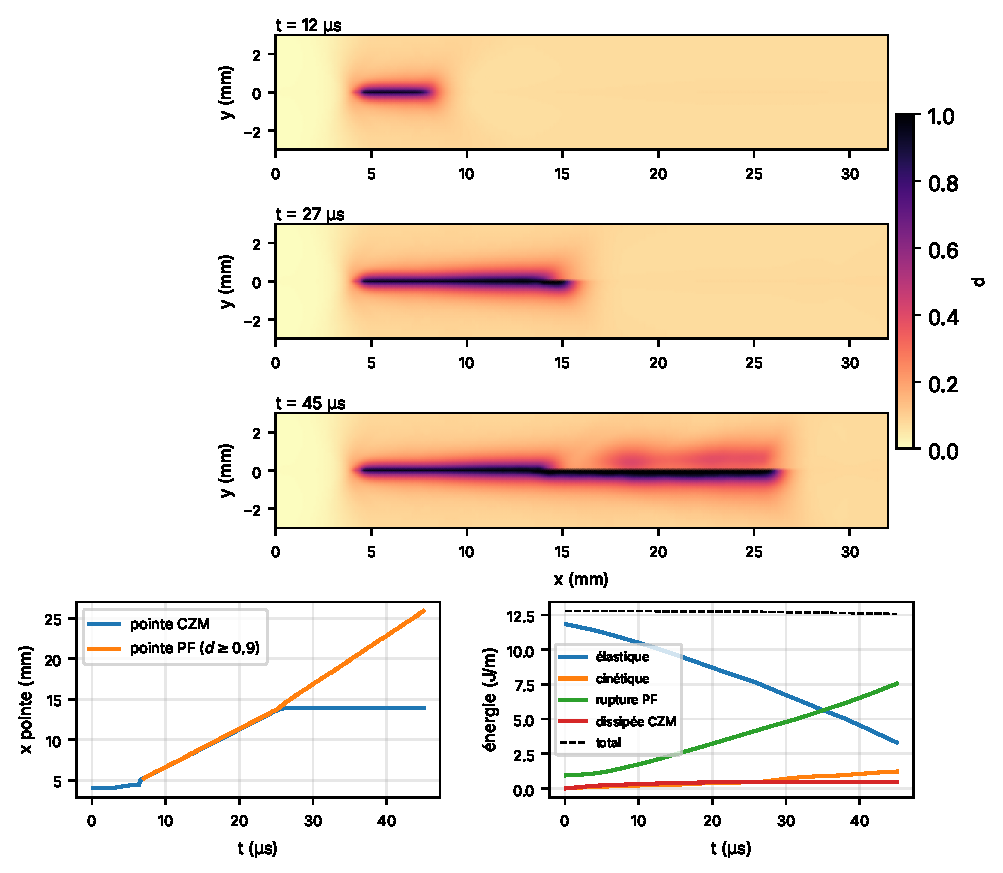
\includegraphics[width=\linewidth]{resultat.pdf}
\caption{Champ de phase à trois instants, position des pointes et bilan d'énergie.}
\end{figure}

\begin{itemize}
\item De 5 à 14~mm, la zone cohésive et le champ de phase avancent ensemble le long de l'interface, à
environ $0{,}55\,c_R$.
\item Vers 14~mm, le champ de phase quitte l'interface et se propage seul juste en dessous, à environ
$0{,}65\,c_R$.
\item La dissipation par unité d'avancée reste entre $0{,}8$ et $1{,}2\,G_c$ pendant la propagation. La
zone cohésive dissipe $0{,}5$~J/m, le champ de phase $7{,}5$~J/m.
\item L'énergie totale baisse de 1{,}7~\%, ce qui est cohérent avec l'amortissement numérique de HHT-$\alpha$.
Newton converge en 5 à 8 itérations cumulées par pas, sans division du pas.
\end{itemize}

\section{Limites}
\begin{itemize}
\item Le maillage de démonstration est grossier ($\ell_0=0{,}4$~mm contre $0{,}1$~mm chez Bleyer) ; la
convergence en maillage n'a pas été étudiée.
\item Avec AT2 et cette valeur de $\ell_0$, la pré-déformation endommage tout le volume d'environ 7~\%.
\item L'état initial est un équilibre élastique à $d=0$ : le premier pas crée une petite onde parasite.
\item Les modes I et II ont la même raideur et la même loi ; il n'y a pas de critère de Benzeggagh-Kenane.
Une mixité variable rendrait la tangente non symétrique.
\item La sortie d'interface à 14~mm peut dépendre du choix $d^+\neq d^-$ ; l'option \texttt{tie\_d} n'a pas
été explorée sur un calcul complet.
\item Maillage Q4 structuré, alors que Bleyer utilise des triangles : un biais sur le branchement est possible.
\end{itemize}

\section{Paramètres principaux}
\begin{center}
\begin{tabular}{lll}
\toprule
Option & Défaut & Rôle\\
\midrule
\texttt{l0}, \texttt{h} & $0{,}1$~mm, $\ell_0/4$ & longueur interne, taille de maille fine\\
\texttt{dU} & $0{,}035$~mm & déplacement imposé\\
\texttt{x\_czm\_end} & $L$ & fin de l'interface cohésive\\
\texttt{Gc\_i}, \texttt{sig\_i} & $G_c$, $\sqrt{3G_cE/(8\ell_0)}$ & ténacité et résistance de l'interface\\
\texttt{K\_fac} & 2 & pénalité $K=K_{fac}E/h$\\
\texttt{tie\_d} & non & $d$ continu à travers l'interface\\
\texttt{alpha\_hht} & $0{,}05$ & amortissement numérique\\
\texttt{dt\_fac} & 1 & $\Delta t=\mathtt{dt\_fac}\cdot h/c_R$\\
\texttt{newton\_tol}, \texttt{stag\_tol} & $10^{-6}$, $10^{-3}$ & tolérances de Newton et de l'alterné\\
\bottomrule
\end{tabular}
\end{center}

\section*{Références}
\begin{itemize}
\item J.~Bleyer, C.~Roux-Langlois, J.-F.~Molinari, \emph{Dynamic crack propagation with a variational
phase-field model: limiting speed, crack branching and velocity-toughening mechanisms}, Int. J. Fract., 2017.
\item M.~Paggi, J.~Reinoso, \emph{A modeling framework for the interaction between the phase field approach
for brittle fracture and the interface cohesive zone model}, Comput. Methods Appl. Mech. Engrg. 321, 2017.
\item A.~Quintanas-Corominas, A.~Turon, J.~Reinoso \emph{et al.}, \emph{A phase field approach enhanced with
a cohesive zone model for modeling delamination induced by matrix cracking}, Comput. Methods Appl. Mech.
Engrg. 358, 2020.
\end{itemize}
\end{document}
